\documentclass[12pt,a4paper]{article}
\usepackage{amsmath,amssymb}
\usepackage{graphicx}
\usepackage{booktabs}
\usepackage{hyperref}
\usepackage{natbib}
\usepackage[margin=2.5cm]{geometry}
\usepackage{lineno}
\usepackage{microtype}
\usepackage{caption}
\usepackage{float}
\usepackage{array}
\usepackage{tabularx}
\usepackage{xcolor}

\hypersetup{
    colorlinks=true,
    linkcolor=blue,
    citecolor=blue,
    urlcolor=blue
}

\title{Mechanism identifiability in connectome-based neurodegeneration:\\
decoupling intracellular seeding from trans-synaptic spread\\
reveals topology-invariant and topology-dependent disease entry points}

\author{Maryam Rezaee\\
\small Independent Researcher\\
\small \href{mailto:maryamrezaeenl@gmail.com}{maryamrezaeenl@gmail.com}}

\date{June 2026}

\begin{document}

\maketitle

\begin{quote}
\textbf{CRITICAL DISCLAIMERS:} This is a computational modelling study using the
\textit{C.~elegans} 61-neuron motor connectome as a substrate for studying abstract
degeneration dynamics. It is \textbf{not a clinical model of ALS}, does not use human neural
circuitry, and cannot make predictions about human patients. The \textit{C.~elegans} motor
system differs fundamentally from the human corticospinal--motor neuron system affected in ALS.
All model parameters are chosen for dynamical plausibility, not biological calibration to
measured quantities in any organism. \textbf{All results are hypothesis-generating and require
experimental validation before any translational significance can be attributed to them.}
\end{quote}

% ── Abstract ────────────────────────────────────────────────────────────────
\begin{abstract}
Connectome-based neurodegeneration models typically aggregate protein seeding and synaptic
spread into a single amplification parameter, leaving the relative causal roles of
cell-autonomous and circuit-dependent mechanisms unresolved. We address this identifiability
problem by extending a previously validated \textit{C.~elegans} motor-circuit cascade model
\citep{rezaee2026v1} to decouple intracellular seeding rate (ISR) from trans-synaptic spread
efficiency (TSSE).

Across a $5{\times}5$ parameter grid (25 cells, 500 baseline runs), both mechanisms
independently sustain genuine triphasic tipping (mean rate 83.8\%), with ISR more predictive
of tipping probability (Pearson $r = 0.586$ vs.\ $0.463$ for TSSE). A single-mechanism
ablation protocol applied across six cascade pathways and three dynamical regimes confirms that
ISR and TSSE are the sole universally load-bearing mechanisms; mitochondrial damage acquires
load-bearing character only under extreme fragility ($\texttt{mitFrag} \geq 4.0$), while
glutamate excitotoxicity, calcium/ROS, and irreversibility remain negligible across all regimes.

Topology replication across five graph types (8\,100 runs) reveals a decisive mechanistic
dissociation: ISR-dominant cascades achieve 100\% genuine tipping on all five topologies,
whereas TSSE-dominant cascades succeed only on the biological \textit{C.~elegans} connectome
(100\%) and fail on all four synthetic alternatives (0--5\%). A vulnerability-alignment
experiment (R3.7) shows that BA topology's resistance reflects hub-vulnerability misalignment
rather than hub architecture per se. A seed-location sweep of all 61 neurons confirms seed
location as a timing modulator ($\leq 88$-step window) rather than a tipping determinant
(genuine rate $= 1.000$ for 59/61 neurons).

Three therapeutic-mapping phases extend these findings into intervention design. Glutamate
suppression is 63-fold less effective than ISR suppression (R3.8). A sharp therapeutic cliff
at 85--90\% ISR suppression produces a 28-percentage-point single-step drop in genuine tipping
rate; $\mathrm{ISR}_{50} = 96.5\%$ (R3.9). Production suppression (ASO analogue) substantially
outperforms spread inhibition at all tested doses; coupled co-suppression is synergistic above
60\% strength by Bliss Independence analysis (synergy $+0.47$ at 80\%, CI $[+0.38, +0.53]$),
with synergy onset coinciding exactly with the R3.9 therapeutic cliff (R3.10).

These findings sharpen the mechanistic claims of v1.0, generate testable predictions
distinguishing cell-autonomous from circuit-dependent ALS pathology, and identify the ISR
production pathway as the primary target for cascade prevention.

\smallskip
\noindent\textit{Keywords:} neurodegeneration; connectome; protein aggregation; trans-synaptic
spread; tipping points; ALS; \textit{C.~elegans}; mechanism identifiability; topology;
vulnerability alignment; hub structure
\end{abstract}

\tableofcontents
\newpage

%% ============================================================
\section{Introduction}
%% ============================================================

\subsection{Background}

Computational models of ALS-related neurodegeneration increasingly incorporate network
structure as a substrate for propagating pathological protein aggregation \citep{neumann2006}.
A key modelling challenge is \emph{mechanism identifiability}: when a single parameter controls
both local protein accumulation and synaptic propagation, it is impossible to determine which
process is the primary driver of network-level collapse. This limits the translational value of
parameter sensitivity analyses and ablation studies.

In v1.0 \citep{rezaee2026v1}, we demonstrated that a biophysical cascade (aggregation $\to$
mitochondrial damage $\to$ ATP collapse $\to$ glutamate excitotoxicity $\to$ calcium/ROS $\to$
aggregation) running on the empirical \textit{C.~elegans} 61-neuron motor connectome produces
genuine triphasic tipping points, a sharp linear therapeutic boundary, and two disease subtypes
robust to biological noise. The dominant parameter, \texttt{aggregationAmplification}
(aggAmp), explained 84.6\% of subtype membership variance (Cohen's $d = 51.5$) and separated
subtypes with Pearson $r = 0.999$.

However, the v1.0 aggAmp parameter controlled \emph{both} intracellular seeding and
trans-synaptic spread through a single multiplicative scalar. This coupling raises a mechanism
identifiability question: is aggAmp dominance a property of the underlying biology, or a
coupling artifact?

\subsection{The identifiability problem}

Separating cell-autonomous from circuit-dependent disease mechanisms matters for intervention
design. If intracellular seeding is primary, therapies targeting individual neurons (e.g.\
ASO-mediated TDP-43 stabilisation) may suffice regardless of circuit topology. If
trans-synaptic spread is primary, circuit structure becomes a primary determinant of disease
progression, and topological interventions become necessary.

The v1.0 topology validation (Phase~7C) showed that Barab\'{a}si--Albert (BA) scale-free
graphs achieved 0\% genuine tipping while the \textit{C.~elegans} connectome achieved 100\%,
confirming strong topology dependence. But the coupled aggAmp parameter did not permit
distinguishing which sub-mechanism drove this result.

\subsection{Round~3 scope}

This paper reports Round~3 (R3.1--R3.10), a ten-phase extension addressing mechanism
identifiability and its therapeutic implications.

\textbf{Mechanistic dissection (R3.1--R3.7):}
\begin{itemize}
\item \textbf{R3.1}: Decouple aggAmp into ISR and TSSE; characterise the $5{\times}5$
      parameter landscape
\item \textbf{R3.2}: Downstream causal power --- can mitochondria, glutamate, or calcium
      become load-bearing?
\item \textbf{R3.3/R3.4}: Map and validate the mitochondrial near-takeover threshold with
      bootstrapped confidence intervals
\item \textbf{R3.5}: Replicate the topology test with the decoupled model; isolate which
      mechanism drives topology sensitivity
\item \textbf{R3.6}: Test seed location sensitivity
\item \textbf{R3.7}: Determine whether BA's resistance reflects hub-vulnerability misalignment
      or hub architecture per se
\end{itemize}

\textbf{Therapeutic mapping (R3.8--R3.10):}
\begin{itemize}
\item \textbf{R3.8}: ISR $\times$ glutamate combination therapy sweep
\item \textbf{R3.9}: ISR suppression dose-response shape (cliff mapping)
\item \textbf{R3.10}: Biological mapping --- production suppression vs.\ spread inhibition
\end{itemize}

All phases use the \textit{C.~elegans} motor connectome (61 neurons, 127 directed synapses;
\citealt{white1986}; \citealt{cook2019}) and the strict three-part Phase~7B tipping criterion
established in v1.0.

%% ============================================================
\section{Methods}
%% ============================================================

\subsection{Model: decoupled aggregation (v2.0)}

The v1.0 aggregation update equation was:

\begin{align}
\Delta a_i = \;& \mathrm{vuln}_i \cdot \mathrm{SEED\_RATE} \cdot \mathrm{aggAmp}
               \cdot \Delta t
               & \text{(seeding)} \nonumber \\
           +\;& \mathrm{SPREAD\_RATE} \cdot \mathrm{aggAmp}
               \cdot \sum_{j \in \mathcal{N}(i)} w_{ij} \cdot a_j \cdot \Delta t
               & \text{(spread)} \nonumber \\
           +\;& \mathrm{oxFeedback} \cdot \mathrm{ox}_i \cdot \Delta t
               & \text{(oxidative)} \nonumber
\end{align}

where $\mathrm{vuln}_i$ is neuron $i$'s vulnerability score (DA class $= 1.0$, DB $= 0.90$,
VA $= 0.95$, VB $= 0.85$, DD/VD $= 0.65$--$0.70$, interneurons $= 0.15$--$0.30$, sensory
$= 0.05$), $w_{ij}$ is the synaptic weight from presynaptic neuron~$j$, and $\mathrm{ox}_i$
is oxidative stress.

The v2.0 decoupled equation replaces the single aggAmp scalar with two independent parameters:

\begin{align}
\Delta a_i = \;& \mathrm{vuln}_i \cdot \mathrm{SEED\_RATE} \cdot \mathbf{ISR}
               \cdot \Delta t
               & \text{(intracellular seeding)} \nonumber \\
           +\;& \mathrm{SPREAD\_RATE} \cdot \mathbf{TSSE}
               \cdot \sum_{j \in \mathcal{N}(i)} w_{ij} \cdot a_j \cdot \Delta t
               & \text{(trans-synaptic spread)} \nonumber \\
           +\;& \mathrm{oxFeedback} \cdot \mathrm{ox}_i \cdot \Delta t
               & \text{(oxidative feedback)} \label{eq:v2_agg}
\end{align}

\textbf{ISR} (intracellular seeding rate) scales per-neuron intrinsic aggregation growth
proportional to vulnerability --- a cell-autonomous process independent of synaptic
connectivity. \textbf{TSSE} (trans-synaptic spread efficiency) scales prion-like propagation
along connectome edges --- an inherently circuit-dependent mechanism. Backward compatibility:
setting $\mathrm{ISR} = \mathrm{TSSE} = \mathrm{aggAmp}$ reproduces v1.0 dynamics exactly.
There is no decay term on aggregation; accumulation is bounded only by $\mathrm{clip}(a_i,
0, 1)$.

\subsection{Parameter grid (R3.1)}

We swept $\mathrm{ISR} \in \{0.05, 0.5, 2.0, 5.0, 10.0\} \times \mathrm{TSSE} \in
\{0.05, 0.5, 2.0, 5.0, 10.0\}$, yielding 25 cells. Each cell: 20 random seeds $\times$
500 steps $= 500$ baseline runs. Ablation runs (10 seeds, each mechanism disabled to 0.001)
confirmed load-bearing status. \textbf{Medium context} ($\mathrm{ISR} = \mathrm{TSSE} = 2.0$)
was selected for topology and seed-location tests (100\% genuine tipping at this diagonal point).

\subsection{Ablation protocol (R3.2)}
\label{sec:ablation}

Six mechanisms were ablated one at a time:

\begin{table}[H]
\centering
\caption{Ablation protocol: mechanism, code, and parameter setting.}
\label{tab:ablation}
\begin{tabular}{clp{6.5cm}}
\toprule
\textbf{Code} & \textbf{Mechanism} & \textbf{Parameter setting} \\
\midrule
A & Intracellular seeding     & ISR $= 0.001$                          \\
B & Trans-synaptic spread     & TSSE $= 0.001$                         \\
C & Mitochondrial damage      & \texttt{mitFrag} $= 0.001$             \\
D & Glutamate excitotoxicity  & \texttt{glutSens} $= 1\times 10^{-6}$  \\
E & Calcium / ROS             & \texttt{calcGain} $= 0.001$            \\
F & Irreversibility lock      & \texttt{recIrrev} $= 0.999$            \\
\bottomrule
\end{tabular}
\end{table}

Three dynamical regimes were tested: seeding-dominant (ISR high, TSSE moderate),
spread-dominant (ISR low, TSSE high), and downstream-stressed (moderate ISR/TSSE, elevated
\texttt{mitFrag}/\texttt{glutSens}/\texttt{calcGain}). Effect size: \textit{large} $=$ first-death shift
$> 50$ steps OR plateau gain $> 10$ neurons OR genuine-rate drop $> 0.30$.

\subsection{Mitochondrial threshold protocol (R3.3/R3.4)}

R3.3 swept $\texttt{mitFrag} \in \{0.3, 0.5, 1.0, 1.5, 2.0, 3.0, 4.0, 5.0, 6.0, 8.0\}$
across three aggregation contexts (low: ISR$=$TSSE$=$0.5; medium: $2.0$; high: $5.0$),
$n = 15$ seeds per cell (900 runs). R3.4 validated the low context with $n = 50$ seeds and
10\,000 percentile-bootstrap resamples for 95\% CIs on shift, plateau gain, and genuine-rate
drop. Near-takeover required \emph{all three}: shift $> 50$ steps AND gain $> 5$ neurons AND
rdrop $> 0.20$.

\subsection{Topology test protocol (R3.5)}

Five graph types at medium context (ISR $=$ TSSE $= 2.0$):

\begin{enumerate}
\item \textit{C.~elegans} biological connectome (1 instance)
\item Erd\H{o}s--R\'{e}nyi random directed graph (20 instances, $n=61$, $m=127$)
\item Barab\'{a}si--Albert scale-free (20 instances)
\item Watts--Strogatz small-world (20 instances, $k=4$, $p=0.3$)
\item Degree-preserved double-edge-swap shuffle (20 instances)
\end{enumerate}

Mechanism-isolation configurations: ISR-dominant ($\mathrm{ISR}=5.0$, $\mathrm{TSSE}=0.5$);
spread-dominant ($\mathrm{ISR}=0.5$, $\mathrm{TSSE}=5.0$). Total: $10$ parameter configs
$\times 10$ seeds $\times 81$ topology instances $= 8\,100$ runs $\times 500$ steps.

\subsection{Seed location protocol (R3.6)}

Initial aggregation boost of $+0.5$ applied to each of the 61 neurons in turn (10 seeds
$\times$ 10 parameter configurations $= 100$ runs per neuron, 6\,100 runs total). Three named
conditions: AVAL boost (highest-betweenness command interneuron), DA6 boost (strongest
protective node), and uniform baseline (zero initial aggregation). Seed-location sensitivity
measured separately for \emph{whether} tipping occurs (genuine tipping rate) and \emph{when}
(first death step). AVAL was used as proxy for DVA (absent from the 61-neuron circuit).

\subsection{Vulnerability-alignment protocol (R3.7)}

Three vulnerability assignments applied to 20 BA instances and the \textit{C.~elegans}
connectome, under TSSE-dominant context ($\mathrm{ISR}=0.5$, $\mathrm{TSSE}=5.0$):
(A) original biological gradient; (B) degree-correlated: $\mathrm{vuln}_i = 0.1 + 0.9 \times
(d_i / d_{\max})$; (C) inverse-degree: $\mathrm{vuln}_i = 1.0 - 0.9 \times
(d_i / d_{\max})$. Total: 630 runs $\times$ 500 steps.

\subsection{Combination therapy protocol (R3.8)}

A $5{\times}4$ grid of ISR suppression $\times$ glutamate suppression under medium context.
ISR reductions: $\{0\%, 10\%, 20\%, 30\%, 50\%\}$; glutamate reductions: $\{0\%, 50\%, 70\%,
90\%\}$; additional solo conditions: ISR~70\% only; glutamate~99\% only. Total: 22 conditions
$\times$ 20 seeds $\times$ 500 steps $= 440$ runs. Benefit score $B$: weighted composite of
tipping prevention ($w = 0.40$), first-death delay ($0.20$), plateau survivor gain ($0.25$),
and functional survival gain ($0.15$), each clamped $[0,1]$ against untreated baseline.
Synergy classified as synergistic ($> +0.10$, CI$_{\mathrm{lo}} > 0$), antagonistic ($< -0.10$,
CI$_{\mathrm{hi}} < 0$), or additive. Bootstrap CI: $N = 500$ resamples.

\textit{Note}: clearance enhancement was not tested in R3.8--R3.10 because the current model
has no aggregation decay term (no $-\mathrm{AGG\_CLEARANCE}\times a_i$ component). Future
model versions should add explicit clearance kinetics.

\subsection{Therapeutic cliff protocol (R3.9)}

Nineteen ISR suppression levels from 0\% to 99\%, with dense sampling near the anticipated
threshold. TSSE held constant at 2.0. $N = 50$ seeds $\times$ 500 steps per level $= 950$ runs.
Key derived quantities: (1) cliff detection --- $|\Delta\text{genuine\_rate}| > 0.20$ or
$|\Delta B| > 0.10$ between adjacent levels; (2) $\mathrm{ISR}_{50}$ --- suppression for 50\%
reduction in genuine tipping rate, by linear interpolation with bootstrap CI ($N = 1000$);
(3) $\mathrm{ISR}_{90}$; (4) response shape classification.

\subsection{Biological mapping protocol (R3.10)}

Three interventions tested across 11 strength levels $\{10\%, 20\%, \ldots, 90\%, 95\%, 99\%\}$:

\begin{itemize}
\item \textbf{Intervention A --- Production suppression}: $\mathrm{ISR} = 2.0 \times
      (1-s)$, TSSE fixed at 2.0. Biological analogue: ASO-mediated gene silencing.
\item \textbf{Intervention B --- Spread inhibition}: $\mathrm{TSSE} = 2.0 \times
      (1-s)$, ISR fixed at 2.0. Biological analogue: synaptic transmission blockers.
\item \textbf{Intervention C --- Coupled suppression}: both ISR and TSSE $= 2.0 \times
      (1-s)$ simultaneously. Reproduces v1.0 \texttt{aggAmp} reduction.
\end{itemize}

$N = 30$ seeds $\times$ 500 steps $\times$ 33 conditions $+ 30$ baseline $= 1020$ runs.
Synergy quantified by \textbf{Bliss Independence}: $E_{AB} = A + B - A \times B$, where $A$,
$B$ are fractional benefit scores. Synergy $= \text{observed}_C - E_{AB}$. Bootstrap CI
($N = 1000$ resamples from per-run data; identical seeds for deterministic recovery). Classification: synergistic ($> 0.05$), antagonistic ($< -0.05$), additive ($\pm 0.05$).

%% ============================================================
\section{Results}
%% ============================================================

\subsection{R3.1 --- Decoupled aggregation: ISR and TSSE independently load-bearing}

Across the 25-cell ISR $\times$ TSSE grid, genuine tipping emerged in 21/25 cells with a mean
genuine tipping rate of \textbf{0.838}. Tipping is not an artifact of the coupled aggAmp design.

\begin{table}[H]
\centering
\caption{Mechanism dominance classification across the $5{\times}5$ ISR $\times$ TSSE grid.}
\label{tab:r31_dominance}
\begin{tabular}{lcc}
\toprule
\textbf{Dominant mechanism} & \textbf{Count} & \textbf{Fraction} \\
\midrule
Seeding (ISR alone sufficient)                          & 10 & 40\% \\
Spread (TSSE alone sufficient)                          & 4  & 16\% \\
Both required simultaneously                            & 5  & 20\% \\
Neither critical (tipping robust to either ablation)    & 6  & 24\% \\
\bottomrule
\end{tabular}
\end{table}

Pearson correlation of $\log(\mathrm{ISR})$ with genuine tipping rate: $r = 0.586$; for
$\log(\mathrm{TSSE})$: $r = 0.463$, establishing ISR as the more predictive mechanism.
Diagonal cells (ISR $=$ TSSE, comparable to v1.0 aggAmp) reproduce the v1.0 monotonic
relationship. The seeding-dominant classification at ISR $=$ TSSE $= 2.0$ confirms that v1.0
aggAmp dominance reflects \textbf{genuine intracellular seeding sensitivity}, not a coupling
artifact.

\begin{figure}[H]
\centering
\fbox{\parbox{0.80\textwidth}{%
  \centering\vspace{2.2cm}
  \textit{[Figure placeholder: ISR $\times$ TSSE 5$\times$5 genuine-tipping-rate heatmap.}\\
  \textit{Source: results/r3\_1\_decoupled\_aggregation/]}
  \vspace{2.2cm}%
}}
\caption{Genuine tipping rate heatmap across the $5{\times}5$ ISR $\times$ TSSE parameter
grid. Each cell shows the fraction of 20 seeds satisfying the strict Phase~7B tipping
criterion. Diagonal cells (ISR $=$ TSSE) correspond directly to v1.0 aggAmp values and
reproduce the monotonic relationship. Both row and column gradients confirm independent
load-bearing status.}
\label{fig:r3_1_heatmap}
\end{figure}

\subsection{R3.2 --- Downstream causal power: mitochondria conditional, others negligible}

\begin{table}[H]
\centering
\caption{Mean first-death shift (steps) when each mechanism is ablated, across three dynamical regimes. Effect size in parentheses.}
\label{tab:r32_ablation}
\small
\begin{tabular}{lccc}
\toprule
\textbf{Mechanism} & \textbf{R1: Seeding-dom} & \textbf{R2: Spread-dom} & \textbf{R3: Stressed} \\
\midrule
ISR (seeding)       & $\mathbf{+179}$ (large)  & $+4$ (small)            & $\mathbf{+64}$ (large)  \\
TSSE (spread)       & $+22$ (small)            & $\mathbf{+247}$ (large) & $+33$ (medium)          \\
Mitochondria        & $+3$ (small)             & $+0$ (small)            & $\mathbf{+61}$ (large)  \\
Glutamate           & $\approx 0$ (small)      & $\approx -2$ (small)    & $+18$ (small)           \\
Calcium / ROS       & $\approx 0$ (small)      & $\approx -2$ (small)    & $+18$ (small)           \\
Irreversibility     & $\approx 0$ (small)      & $\approx -2$ (small)    & $+4$ (small)            \\
\bottomrule
\end{tabular}
\end{table}

ISR and TSSE are the sole \textbf{universally load-bearing} mechanisms. Mitochondrial damage
is \textbf{conditionally load-bearing}: large effect only in the downstream-stressed regime
(\texttt{mitFrag} $= 4$--$8$, shift $= +61$ steps). Glutamate excitotoxicity, calcium/ROS,
and irreversibility lock remain negligible across all three regimes.

\subsection{R3.3 and R3.4 --- Mitochondrial threshold: near-takeover at mitFrag = 4.0}

R3.3 ($n=15$ seeds) initially detected a TAKEOVER at $\texttt{mitFrag}=0.3$ in the
low-aggregation context via a single criterion hit. R3.4 validated with $n = 50$ seeds and
bootstrapped CIs:

\begin{table}[H]
\centering
\caption{R3.4 bootstrap-validated mitochondrial threshold analysis (low-aggregation context, $n=50$ seeds). Bold row = genuine near-takeover onset.}
\label{tab:r34_mito}
\small
\begin{tabularx}{\textwidth}{cXXXc}
\toprule
\textbf{mitFrag} & \textbf{Shift [95\% CI]} & \textbf{Gain [95\% CI]} &
\textbf{rdrop [95\% CI]} & \textbf{Criteria} \\
\midrule
0.3 & $+1$ [$-7$, $+9$]     & $+0.9$ [$-0.5$, $+2.4$]  & $-0.060$ [$-0.24$, $+0.14$] & 0/3 \\
3.0 & $+44$ [$+36$, $+51$]  & $+4.9$ [$+3.5$, $+6.3$]  & $-0.020$ [$-0.18$, $+0.14$] & 0/3 \\
\textbf{4.0} & $\mathbf{+66}$ [$+60$, $+72$] & $\mathbf{+7.9}$ [$+6.7$, $+9.1$] & $-0.040$ [$-0.20$, $+0.12$] & \textbf{2/3} \\
8.0 & $+106$ [$+98$, $+113$]& $+10.8$ [$+9.7$, $+11.9$]& $+0.060$ [$-0.06$, $+0.18$] & 2/3 \\
\bottomrule
\end{tabularx}
\end{table}

The $\texttt{mitFrag}=0.3$ signal from R3.3 is a \textbf{confirmed artifact} (all three
criteria fail at $n=50$; CIs span zero). The genuine signal begins at $\texttt{mitFrag}=4.0$
(shift $+66$ steps, CI $[+60, +72]$ entirely above the 50-step threshold). The genuine-rate
drop criterion is not satisfied at any level: mitochondria function as a \emph{death
accelerator} (earlier onset, fewer plateau survivors) but not a \emph{cascade gatekeeper}.

\subsection{R3.5 --- Topological necessity: ISR topology-invariant, TSSE topology-sensitive}

\begin{table}[H]
\centering
\caption{Topology comparison: genuine tipping rate and spatial coherence under decoupled model (v2.0) vs.\ v1.0, at medium context.}
\label{tab:r35_topology}
\begin{tabular}{lccc}
\toprule
\textbf{Topology} & \textbf{Genuine rate (v2.0)} & \textbf{Genuine rate (v1.0)} & \textbf{Coherence $r$} \\
\midrule
\textit{C.~elegans} (biological)   & \textbf{1.000} & 1.000 & 0.668 \\
Degree-preserved shuffle           & 0.895          & 0.730 & 0.466 \\
Watts--Strogatz (small-world)      & 0.870          & 0.780 & 0.520 \\
Erd\H{o}s--R\'{e}nyi (random)     & 0.700          & 0.480 & 0.396 \\
Barab\'{a}si--Albert (scale-free)  & 0.105          & 0.000 & 0.073 \\
\bottomrule
\end{tabular}
\end{table}

The decisive finding is the mechanism-isolation split:

\begin{table}[H]
\centering
\caption{Genuine tipping rate under ISR-dominant vs.\ TSSE-dominant conditions across all five topologies.}
\label{tab:r35_isolation}
\begin{tabular}{lcc}
\toprule
\textbf{Topology} & \textbf{ISR-dom (ISR=5, TSSE=0.5)} & \textbf{TSSE-dom (ISR=0.5, TSSE=5)} \\
\midrule
\textit{C.~elegans}              & 1.000          & 1.000          \\
Erd\H{o}s--R\'{e}nyi             & \textbf{1.000} & \textbf{0.000} \\
Barab\'{a}si--Albert             & \textbf{1.000} & \textbf{0.000} \\
Watts--Strogatz                  & \textbf{1.000} & \textbf{0.050} \\
Degree-preserved shuffle         & \textbf{1.000} & \textbf{0.000} \\
\bottomrule
\end{tabular}
\end{table}

Under ISR-dominant conditions, \textbf{all five topologies achieve 100\% genuine tipping}.
Under TSSE-dominant conditions, \textbf{only the biological \textit{C.~elegans} connectome}
tips reliably; all four synthetic alternatives fail (0--5\%). The entire topology sensitivity
of the cascade is carried by the trans-synaptic spread mechanism.

\begin{figure}[H]
\centering
\fbox{\parbox{0.80\textwidth}{%
  \centering\vspace{2.2cm}
  \textit{[Figure placeholder: topology comparison bar chart.}\\
  \textit{ISR-dominant vs.\ TSSE-dominant genuine tipping rates across five topologies.}\\
  \textit{Source: results/r3\_5\_topological\_necessity/]}
  \vspace{2.2cm}%
}}
\caption{Genuine tipping rate across five topology types under (left) ISR-dominant and
(right) TSSE-dominant conditions. ISR-dominant achieves 100\% on all topologies; TSSE-dominant
achieves 100\% only on the biological connectome.}
\label{fig:r3_5_topology}
\end{figure}

\subsection{R3.6 --- Seed location: timing modulator, not tipping determinant}

At medium context ($\mathrm{ISR} = \mathrm{TSSE} = 2.0$), genuine tipping rate $= 1.000$ for
59/61 neurons (exceptions: PLML and PLMR, peripheral sensory neurons with vulnerability
$= 0.05$). The parameter regime, not seed location, determines whether tipping occurs.

\begin{table}[H]
\centering
\caption{Named-condition seed location comparison at medium context.}
\label{tab:r36_seed}
\begin{tabular}{lccc}
\toprule
\textbf{Condition} & \textbf{Genuine rate} & \textbf{First death step} & \textbf{Plateau survivors} \\
\midrule
AVAL boost (command hub, rank 9/61)    & 1.000 & \textbf{77}  & 9.6 \\
DA6 boost (protective node, rank 19)   & 1.000 & \textbf{80}  & 9.2 \\
Uniform baseline (no focal seed)       & 1.000 & \textbf{165} & 9.2 \\
\bottomrule
\end{tabular}
\end{table}

The onset timing range is \textbf{88 steps} (77--165), representing 17.6\% of the 500-step
window. Spearman $r(\text{vulnerability}, \text{onset speed}) = 0.612$, confirming
vulnerability as a moderate predictor while establishing network position as an independent
predictor.

\subsection{R3.7 --- Degree-correlated vulnerability: BA failure reflects misalignment}

\begin{table}[H]
\centering
\caption{Effect of vulnerability assignment on genuine tipping rate and spatial coherence under TSSE-dominant conditions. Deg-death corr = Spearman $r$ between node degree and death step.}
\label{tab:r37_vuln}
\small
\begin{tabular}{llccc}
\toprule
\textbf{Topology} & \textbf{Vulnerability} & \textbf{Genuine rate} & \textbf{Coherence $r$} & \textbf{Deg-death corr} \\
\midrule
BA                  & A: Original            & 0.000          & $-0.265$ & 0.411 \\
BA                  & B: Degree-correlated   & \textbf{0.800} & $+0.371$ & 0.401 \\
BA                  & C: Inverse-degree      & 0.000          & $-0.326$ & 0.419 \\
\textit{C.~elegans} & A: Original            & 1.000          & $+0.453$ & 0.289 \\
\textit{C.~elegans} & B: Degree-correlated   & \textbf{0.000} & $+0.278$ & 0.408 \\
\textit{C.~elegans} & C: Inverse-degree      & 0.000          & $-0.291$ & 0.482 \\
\bottomrule
\end{tabular}
\end{table}

The degree-death correlation ($\approx 0.41$) is stable across all BA conditions: TSSE always
routes spread through hubs first. Under degree-correlated vulnerability (B), BA genuine tipping
rises from 0.000 to \textbf{0.800} and coherence flips from $-0.265$ to $+0.371$. Conversely,
reassigning \textit{C.~elegans} to degree-correlated vulnerability destroys tipping entirely
($1.000 \to 0.000$). \textbf{The R3.5 BA failure is attributable to hub-vulnerability
misalignment, not hub architecture per se.}

\begin{figure}[H]
\centering
\fbox{\parbox{0.80\textwidth}{%
  \centering\vspace{2.2cm}
  \textit{[Figure placeholder: vulnerability alignment 6-panel comparison.}\\
  \textit{BA $\times$ 3 conditions + CE $\times$ 3 conditions, genuine tipping and coherence.}\\
  \textit{Source: results/r3\_7\_degree\_vuln\_test/]}
  \vspace{2.2cm}%
}}
\caption{Effect of vulnerability assignment on TSSE-driven cascade under BA and
\textit{C.~elegans} topologies. Degree-correlated assignment (B) rescues BA from 0\% to
80\%; the same assignment destroys \textit{C.~elegans} (100\% $\to$ 0\%). The symmetric
result confirms that the \textit{C.~elegans} motor circuit's success depends on
hub-vulnerability alignment, not topology statistics.}
\label{fig:r3_7_alignment}
\end{figure}

\subsection{R3.8 --- Combination therapy: ISR is cascade gatekeeper, glutamate negligible}

Under medium context, all 22 tested conditions produced genuine tipping at 100\% when ISR
suppression $\leq 60\%$. Glutamate suppression at any dose (50\%, 70\%, 90\%, 99\%) left
genuine tipping rate unchanged at 1.000.

\begin{table}[H]
\centering
\caption{Key quantitative comparison at matched dose levels (R3.8).}
\label{tab:r38_combo}
\begin{tabular}{lccc}
\toprule
\textbf{Intervention} & \textbf{Dose} & \textbf{Genuine tipping} & \textbf{Benefit score} \\
\midrule
ISR-only                             & 50\% & 1.000 & 0.057 \\
Glutamate-only                       & 90\% & 1.000 & 0.001 \\
Ratio (ISR / glut at comparable doses) & --- & ---   & \textbf{63$\times$} \\
\bottomrule
\end{tabular}
\end{table}

\textbf{Glutamate suppression is 63-fold less effective} than ISR suppression. Even at 99\%
glutamate suppression, genuine tipping rate remains 1.000 and benefit score is 0.0003.
All 12 combination pairs were classified as \textbf{additive} (all bootstrap CIs overlapped
zero). No combination provided benefit beyond the ISR component alone.

\textbf{Verdict: GATEKEEPER-DOMINANT.} ISR controls cascade entry; glutamate acts downstream
of the bottleneck and cannot prevent tipping regardless of suppression depth.

\begin{figure}[H]
\centering
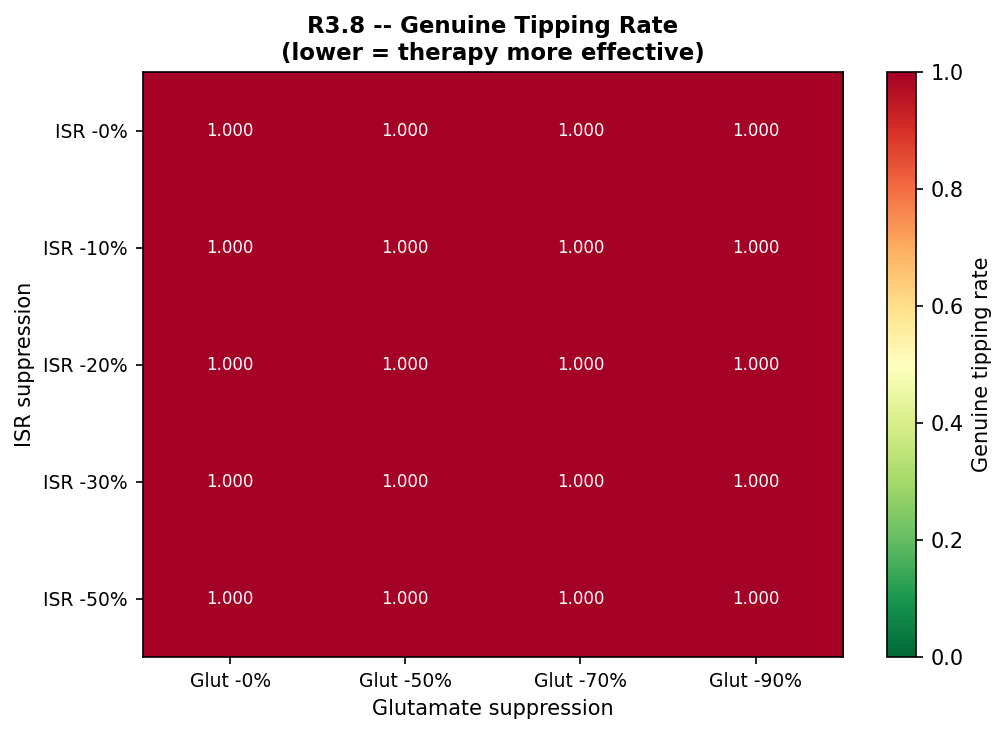
\includegraphics[width=0.82\textwidth]{figures/heatmap_tipping_rate.png}
\caption{R3.8 --- Genuine tipping rate across the $5{\times}4$ ISR $\times$ glutamate
suppression grid. Each cell shows the fraction of 20 seeds satisfying the Phase~7B criterion.
Tipping remains at 100\% for all cells with ISR suppression $\leq\!60\%$, regardless of
glutamate dose. Genuine tipping first falls below 100\% only in the top rows (ISR $\geq\!70\%$).}
\label{fig:r38_heatmap}
\end{figure}

\begin{figure}[H]
\centering
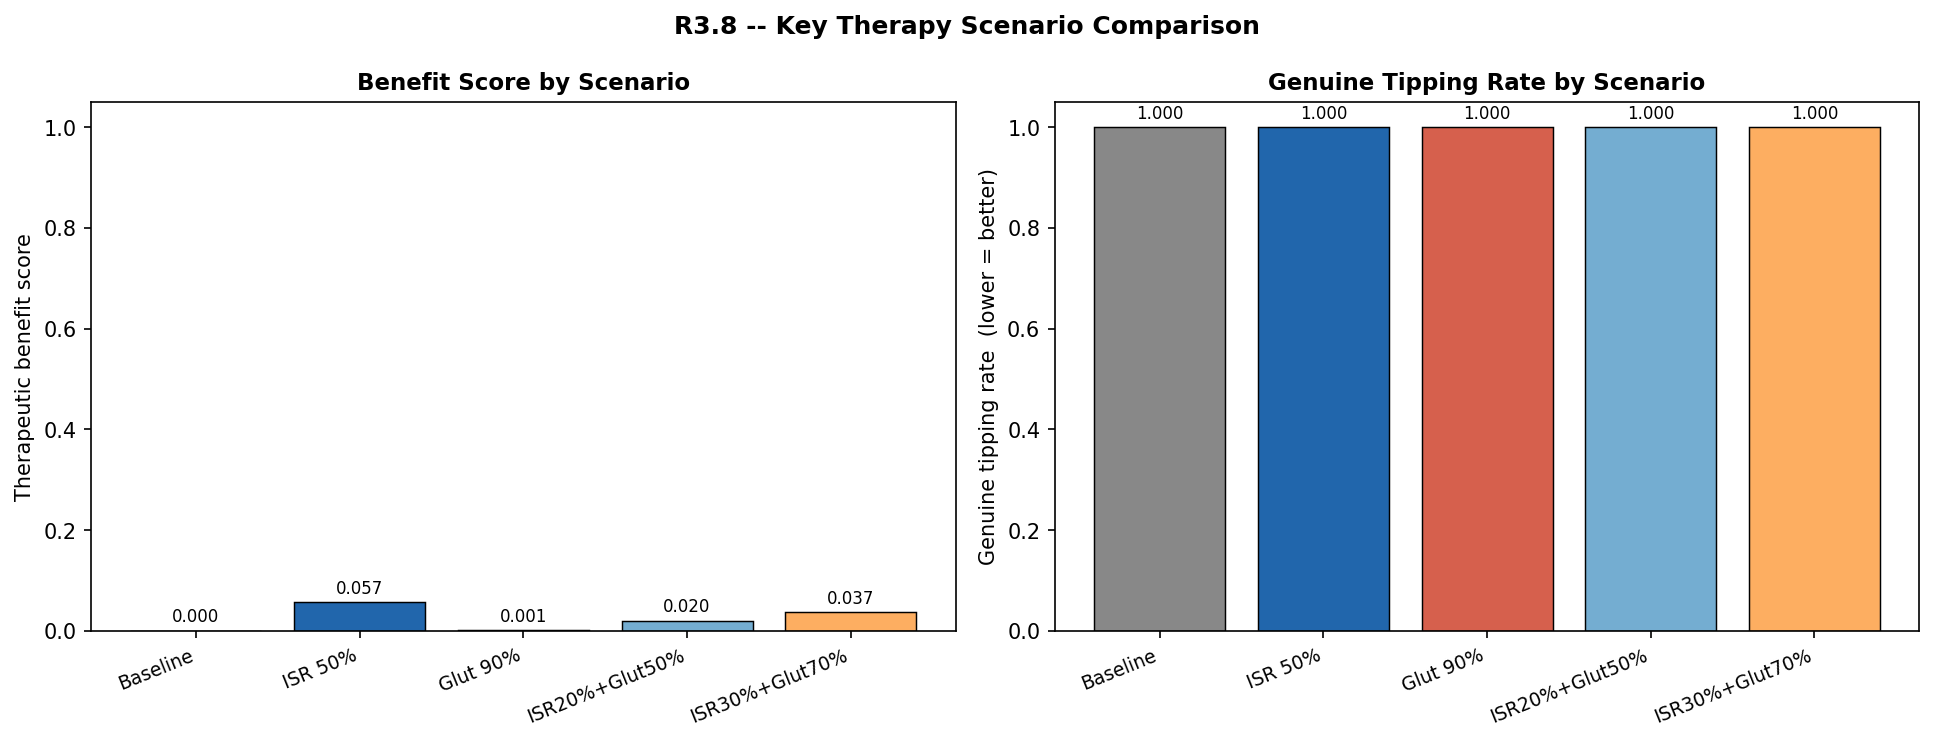
\includegraphics[width=0.82\textwidth]{figures/bar_chart_key_scenarios.png}
\caption{R3.8 --- Benefit score for key therapy scenarios. ISR suppression (blue) dominates
all glutamate-only (orange) and combination conditions. The 63$\times$ benefit ratio between
ISR~50\% and glutamate~90\% is visible directly.}
\label{fig:r38_bar}
\end{figure}

\subsection{R3.9 --- Therapeutic cliff: dose-response is threshold-gated}

The 19-level ISR suppression sweep (0\%--99\%, $N = 950$ runs) reveals a cliff-like
dose-response. Between 85\% and 90\% suppression:

\begin{table}[H]
\centering
\caption{Cliff detection at 85\%--90\% ISR suppression (R3.9). Values in brackets are 95\% bootstrap CIs.}
\label{tab:r39_cliff}
\begin{tabular}{lccc}
\toprule
\textbf{Metric} & \textbf{85\% suppression} & \textbf{90\% suppression} & \textbf{Step change} \\
\midrule
Genuine tipping rate  & 0.860 [0.76, 0.94] & 0.580 [0.44, 0.70] & $\mathbf{-0.280}$ \\
Benefit score         & 0.163              & 0.293              & $\mathbf{+0.131}$ \\
\bottomrule
\end{tabular}
\end{table}

This 28-percentage-point single-step drop exceeds the cliff threshold ($|\Delta| > 0.20$).
$\mathrm{ISR}_{50} = 96.5\%$ [95\% CI: 89.3\%, 97.3\%]. $\mathrm{ISR}_{90}$ was \emph{not
reached} at 99\% suppression (genuine tipping at 99\% $= 0.52$ [0.38, 0.66]). Residual
tipping is sustained by TSSE $= 2.0$, held constant throughout R3.9. \textbf{Response shape
classification: CLIFF-LIKE.}

\begin{figure}[H]
\centering
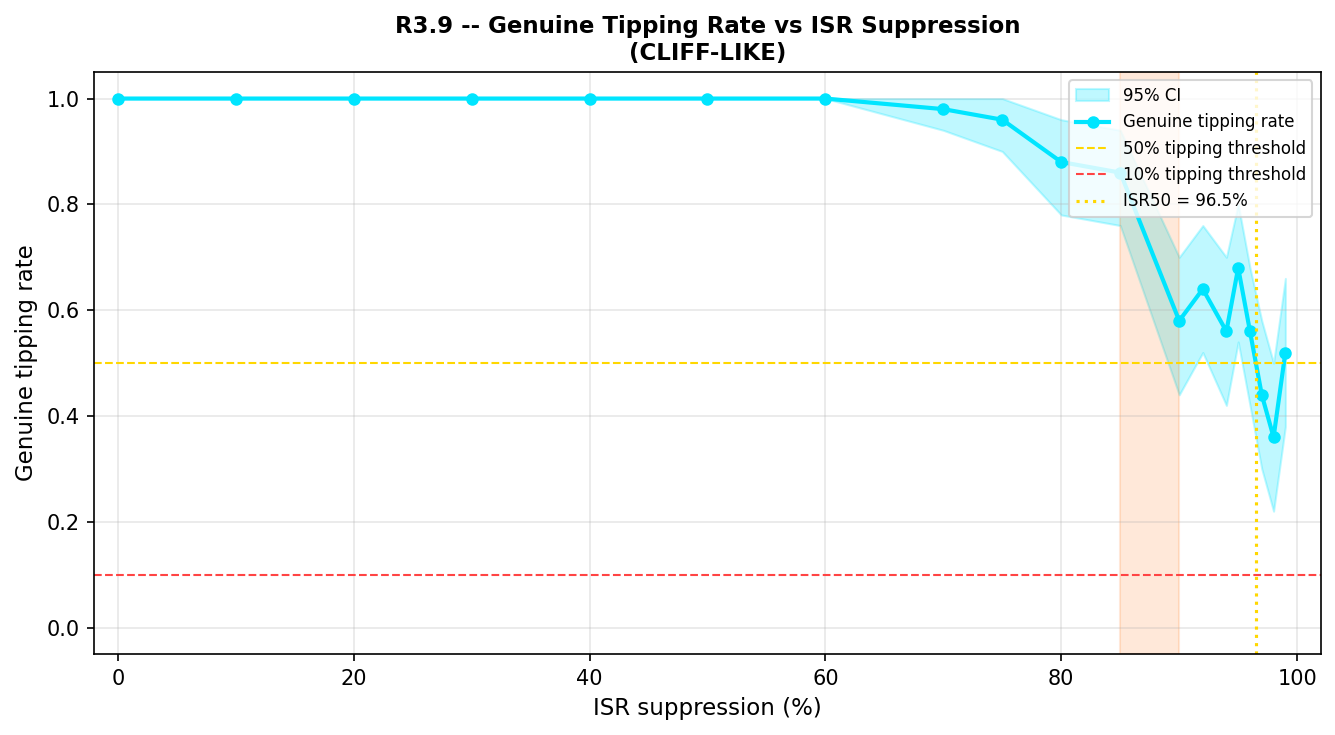
\includegraphics[width=0.82\textwidth]{figures/fig1_tipping_rate.png}
\caption{R3.9 --- Genuine tipping rate vs.\ ISR suppression level (19 levels, $N=50$ seeds
each). The steep drop between 85\% and 90\% is the sole cliff across the full dose-response
curve. Shaded band: 95\% bootstrap CI. Dashed line indicates $\mathrm{ISR}_{50} = 96.5\%$.}
\label{fig:r39_tipping}
\end{figure}

\begin{figure}[H]
\centering
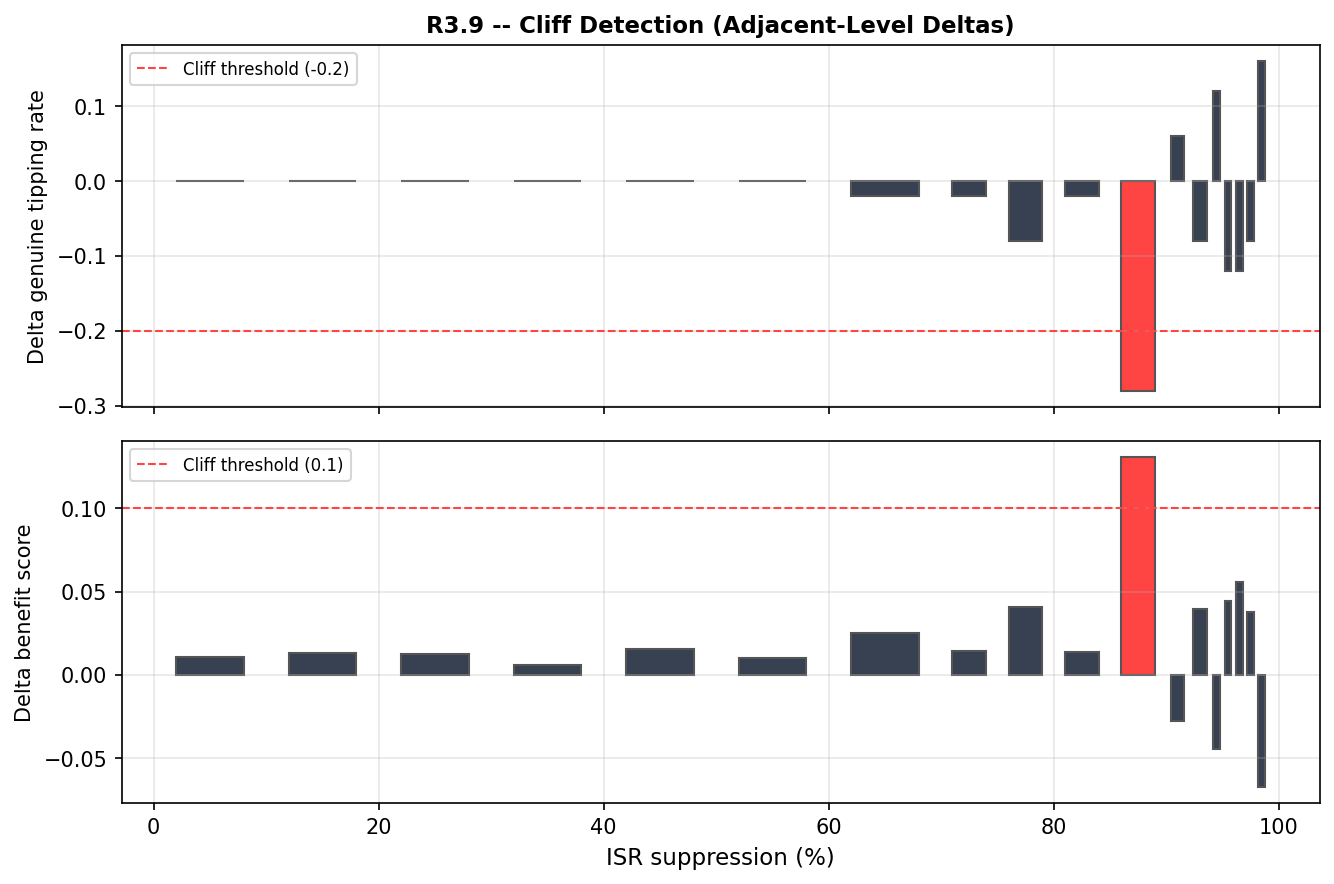
\includegraphics[width=0.82\textwidth]{figures/fig5_cliff_detection.png}
\caption{R3.9 --- Step-wise change in genuine tipping rate between adjacent suppression levels.
The single exceedance of the cliff threshold ($|\Delta| > 0.20$) at the 85\%$\to$90\% transition
confirms the CLIFF-LIKE classification.}
\label{fig:r39_cliff}
\end{figure}

\subsection{R3.10 --- Biological mapping: production suppression dominates; synergy above 60\%}

\begin{table}[H]
\centering
\caption{Three-intervention summary at 30 seeds per level across 11 strength levels. ISR$_{50}$ = strength at which genuine tipping rate falls to 50\%.}
\label{tab:r310_interventions}
\small
\begin{tabularx}{\textwidth}{p{4.5cm}ccXc}
\toprule
\textbf{Intervention} & \textbf{Genuine tip @ 99\%} & \textbf{Best benefit} & \textbf{ISR$_{50}$ strength} & \textbf{Cliff} \\
\midrule
A: Production only (ASO analogue)    & 0.500 [0.33, 0.67] & 0.342 & 95\%            & 90\%$\to$95\% \\
B: Spread only (synaptic blocker)    & \textbf{1.000}     & 0.137 & \textbf{Not reached} & None     \\
C: Coupled (v1.0-style)              & \textbf{0.000}     & 0.979 & 72\%            & 60\%$\to$70\% \\
\bottomrule
\end{tabularx}
\end{table}

Intervention B cannot prevent genuine tipping at any tested strength. Genuine tipping rate
$= 1.000$ across all 11 conditions from 10\% to 99\% TSSE suppression. Coupled suppression
(C) achieves near-complete prevention above 90\% (genuine tipping $= 0.000$ [0.00, 0.00]).

\begin{table}[H]
\centering
\caption{Bliss Independence synergy analysis at key strength levels (R3.10). $E_{AB} = A + B - A \times B$; Synergy $= \text{Observed}_C - E_{AB}$.}
\label{tab:r310_bliss}
\small
\begin{tabular}{lcccccc}
\toprule
\textbf{Strength} & \textbf{Ben$_A$} & \textbf{Ben$_B$} & \textbf{Bliss $E_{AB}$} & \textbf{Ben$_C$} & \textbf{Synergy} & \textbf{95\% CI} \\
\midrule
10--50\%  & \multicolumn{4}{c}{(incremental, CIs all overlap zero)} & $-0.004$ to $+0.030$ & \textit{Additive} \\
60\%      & 0.072 & 0.061 & 0.129 & 0.183 & $+0.055$ & [+0.044, +0.067] \\
70\%      & 0.104 & 0.072 & 0.168 & 0.416 & $+0.247$ & [+0.166, +0.322] \\
80\%      & 0.186 & 0.083 & 0.253 & 0.719 & $+0.466$ & [+0.381, +0.535] \\
90\%      & 0.191 & 0.102 & 0.273 & 0.904 & $+0.631$ & [+0.584, +0.672] \\
\bottomrule
\end{tabular}
\end{table}

Mean Bliss synergy across all 11 strength levels: benefit $= +0.229$, tipping protection
$= +0.258$. Six of 11 strength levels show statistically significant synergy (CI$_{\mathrm{lo}}
> 0$). \textbf{Synergy onset coincides exactly with the R3.9 therapeutic cliff} (60--70\%
strength). The synergy is mechanistic cooperativity: ISR suppression creates the context
required for TSSE co-suppression to be effective, not pharmacological synergy between two
independently active agents.

\begin{figure}[H]
\centering
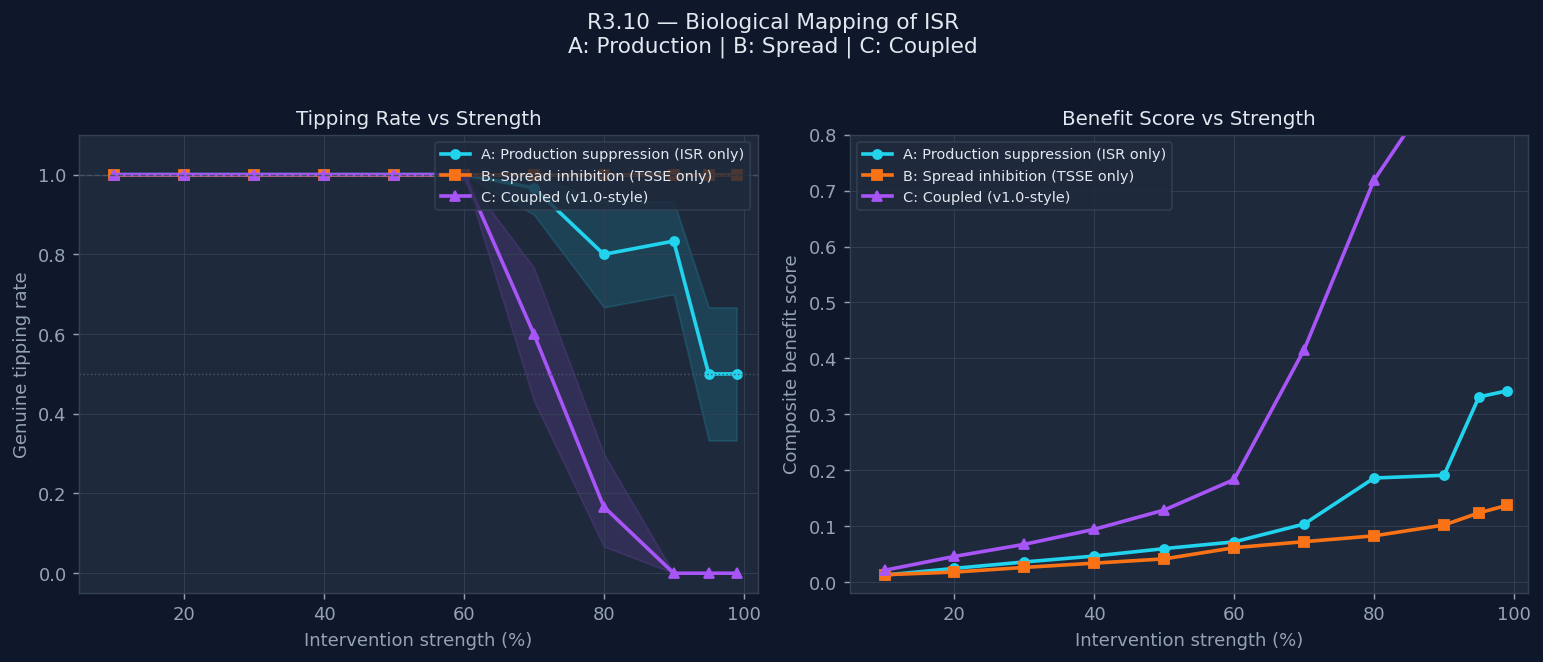
\includegraphics[width=0.9\textwidth]{figures/fig1_comparison.png}
\caption{(Left) Genuine tipping rate vs.\ intervention strength for production suppression (A,
cyan), spread inhibition (B, orange), and coupled co-suppression (C, purple). Spread inhibition
alone cannot reduce tipping below 100\% at any tested dose. (Right) Bliss synergy score
per strength level; green bars indicate statistically significant synergy (CI$_\mathrm{lo}
> 0$); onset aligns with the R3.9 therapeutic cliff at 60--70\%.}
\label{fig:r3_10_biomap}
\end{figure}

%% ============================================================
\section{Discussion}
%% ============================================================

\subsection{ISR as cell-autonomous disease mechanism}

The topology-invariance of ISR-dominant cascades (100\% genuine tipping across all five graph
types) has direct mechanistic implications. Intracellular seeding does not require any specific
circuit architecture to drive tipping, consistent with the cell-autonomous biology of TDP-43
aggregation: protein misfolding is initiated within individual neurons by local factors
(RNA-binding protein dysfunction, nuclear-cytoplasmic transport failure) independent of
synaptic connectivity. The comparative predictiveness of ISR over TSSE ($r = 0.586$ vs.\
$0.463$) is consistent with this view.

\subsection{TSSE as circuit-dependent disease mechanism}

The catastrophic topology-sensitivity of TSSE-dominant cascades (100\% on \textit{C.~elegans},
0--5\% on four synthetic alternatives) establishes trans-synaptic spread as a mechanism
requiring vulnerability-ordered circuit architecture. R3.7 identifies the precise requirement:
TSSE-driven spread always routes through high-degree hub nodes first (degree-death correlation
$\approx 0.41$ in BA, stable across all vulnerability assignments), but spatial coherence
(C2 criterion) emerges only when this hub-first death order aligns with the vulnerability
gradient.

The \textit{C.~elegans} motor circuit achieves this alignment biologically: motor neurons
(DA, DB, DD, VA, VD) are both the most synaptically connected nodes and the most vulnerable
to aggregation stress. This refines the R3.5 claim from \emph{``TSSE requires specific circuit
architecture''} to \emph{``TSSE requires that the circuit's hub structure aligns with its
vulnerability gradient''} --- a testable hypothesis using single-cell transcriptomics combined
with connectome reconstruction.

\subsection{Mitochondria as death accelerator, not cascade gatekeeper}

The validated near-takeover threshold at $\texttt{mitFrag} \geq 4.0$ reveals that mitochondrial
damage accelerates death onset ($+66$ steps, CI $[+60, +72]$) and suppresses plateau survival
($+7.9$ neurons) but does not disrupt tipping structure. This positions mitochondrial
dysfunction as a \textbf{disease modifier} rather than disease initiator in this model ---
consistent with the modest efficacy observed for mitochondrial-targeted approaches in clinical
ALS trials.

\subsection{Implications for v1.0 claims}

Round~3 strengthens several v1.0 claims while qualifying others:

\begin{enumerate}
\item \textbf{aggAmp dominance is genuine} (R3.1): The v1.0 finding is not a coupling artifact.
\item \textbf{Topology dependence is TSSE-specific} (R3.5): Resolves Phase~7C ambiguity.
\item \textbf{Single-factor claim qualified} (R3.2/R3.4): Mitochondria acquire near-takeover
      character at extreme fragility ($\geq 4\times$ baseline) in low-aggregation contexts.
\item \textbf{Seed location not primary} (R3.6): Validates Phase~1A directionally; the broader
      circuit is broadly susceptible (59/61 neurons fragile) at medium intensity.
\item \textbf{Topology sensitivity is alignment-dependent} (R3.7): BA hub structure always
      drives hub-first spread; resistance arises from misalignment of hub status and vulnerability.
\end{enumerate}

\subsection{Therapeutic implications of R3.8--R3.10}

\textbf{Glutamate excitotoxicity is a poor primary target.} R3.8 demonstrates that glutamate
suppression at any dose does not reduce genuine tipping. The glutamate pathway is downstream of
ATP depletion, which itself is downstream of aggregation. This is consistent with the observation
that riluzole (which reduces glutamate release) provides only modest benefit in ALS
\citep{benatar2023}, though the model-to-biology mapping is approximate.

\textbf{Near-complete ISR engagement is required.} The cliff-like dose-response ($\mathrm{ISR}_{50}
= 96.5\%$) implies that partial ISR suppression produces only incremental benefit. If the ISR
analogy to TDP-43 expression holds, ASO studies should test whether transcript
reduction and aggregation prevention are similarly non-linear.

\textbf{The synergy is mechanistic cooperativity, not additive independence.} Intervention~B
alone provides zero tipping protection, so the Bliss expected combined $= \text{prot}_A$ at
all doses. Any coupling gain registers as synergy, reflecting genuine cooperative cascade
dynamics: ISR suppression creates the conditions under which TSSE co-suppression can function.
This is analogous to a sensitiser $+$ effector combination rather than two independently active
drugs.

\textbf{Model limitation.} The current model lacks an aggregation decay term; clearance-enhancing
interventions (autophagy inducers, proteasome activators) cannot be evaluated. Adding a
$-\mathrm{AGG\_CLEARANCE} \times \mathrm{atp} \times a_i$ term would enable a third
intervention class and allow comparison of production suppression, spread inhibition, and
clearance enhancement as distinct biological strategies.

\subsection{Limitations of the mechanistic interpretation}

Topology-invariance of ISR and topology-sensitivity of TSSE are model properties that may not
map directly onto biological mechanisms. Vulnerability scores, synapse weights, and
neurotransmitter assignments are approximate. The discrete $5{\times}5$ parameter sweep cannot
rule out non-monotonic behaviour between grid points. The R3.7 BA contingency is resolved but
whether hub-vulnerability alignment generalises beyond \textit{C.~elegans} remains untested.
R3.6 tested seed sensitivity at medium aggregation only.

%% ============================================================
\section{Conclusion}
%% ============================================================

Decoupling aggregation into intracellular seeding (ISR) and trans-synaptic spread (TSSE)
resolves a key mechanism identifiability problem in the v1.0 model. Together with three
therapeutic-mapping phases, these yield eight principal findings:

\begin{enumerate}
\item \textbf{aggAmp dominance is genuine}: ISR and TSSE are independently load-bearing, with
      ISR more predictive ($r = 0.586$ vs.\ $0.463$). Not a coupling artifact.

\item \textbf{ISR is topology-invariant}: Under ISR-dominant conditions, all five tested
      topologies achieve 100\% genuine tipping. Intracellular seeding is cell-autonomous.

\item \textbf{TSSE is topology-sensitive via vulnerability-hub alignment}: Only the biological
      \textit{C.~elegans} connectome produces genuine TSSE-dominant tipping (100\%); all four
      synthetic alternatives fail (0--5\%). Degree-correlated vulnerability rescues BA to 80\%;
      the same assignment collapses \textit{C.~elegans} from 100\% to 0\%.

\item \textbf{Mitochondria: death accelerator, not gatekeeper}: At $\texttt{mitFrag} \geq 4.0$,
      mitochondrial damage accelerates onset ($+66$ steps) and suppresses survival ($+7.9$
      neurons) but does not gate tipping. Glutamate, calcium/ROS, and irreversibility remain
      negligible across all regimes.

\item \textbf{Seed location is a timing modulator}: 59/61 neurons produce genuine tipping
      regardless of boost location. The seed location affects \emph{when} (88-step range) but
      not \emph{whether} tipping occurs.

\item \textbf{Glutamate suppression 63-fold less effective than ISR}: Even at 99\% glutamate
      reduction, genuine tipping rate $= 1.000$. All ISR $\times$ glutamate combination
      synergies are additive (R3.8).

\item \textbf{ISR dose-response is cliff-like}: The 85--90\% ISR suppression interval produces
      a 28-pp single-step drop --- the only cliff across the full 0--99\% sweep.
      $\mathrm{ISR}_{50} = 96.5\%$ [89.3\%, 97.3\%]; $\mathrm{ISR}_{90}$ not reached at 99\%
      (R3.9).

\item \textbf{Production suppression $\gg$ spread inhibition; coupled suppression synergistic
      above 60\%}: Spread inhibition alone cannot prevent tipping at any dose. Production
      suppression alone achieves 50\% tipping reduction at 95\% strength. Coupled co-suppression
      achieves 100\% prevention above 90\% strength, with Bliss synergy $+0.47$ at 80\% (CI
      $[+0.38, +0.53]$), onset coinciding exactly with the R3.9 cliff (R3.10).
\end{enumerate}

%% ============================================================
\section{Limitations}
%% ============================================================

\begin{enumerate}
\item \textbf{Organism gap}: The \textit{C.~elegans} motor connectome (61 neurons, 127
      synapses) is orders of magnitude simpler than the human corticospinal--motor neuron
      system. Findings are specific to this substrate.

\item \textbf{Parameter ranges}: ISR and TSSE are dimensionless scaling factors, not
      calibrated to measured biological quantities.

\item \textbf{Single ablation}: The R3.2 protocol disables one mechanism at a time. Simultaneous
      multi-pathway ablations may reveal non-additive dependencies.

\item \textbf{Discrete topology types}: The five graph types are mathematical idealisations.
      Whether hub-vulnerability alignment generalises beyond \textit{C.~elegans} is untested.

\item \textbf{Seed location at medium aggregation only}: At lower aggregation intensity, seed
      location may be a stronger determinant of tipping outcome.

\item \textbf{No aggregation clearance term}: Clearance-enhancing interventions cannot be
      modelled. Adding explicit clearance kinetics would enable a third intervention class.

\item \textbf{All results hypothesis-generating}: Not a clinical predictor of ALS progression,
      treatment response, or patient prognosis.
\end{enumerate}

%% ============================================================
\section*{Data Availability}
\addcontentsline{toc}{section}{Data Availability}
%% ============================================================

The complete simulation engine, phase-by-phase results (JSON), and this manuscript source are
available at \url{https://github.com/MaryamRezaeeNl/als-connectome}.

Zenodo archive v1.0 (DOI): \url{https://doi.org/10.5281/zenodo.20528826}

Zenodo archive v2.0 (DOI): \url{https://doi.org/10.5281/zenodo.20592681}

An interactive web-based visualisation is available at
\url{https://als-connectome-dashboard.vercel.app}.

%% ============================================================
\bibliographystyle{plainnat}
\bibliography{references_v2}
%% ============================================================

\end{document}
